\section{Misalignment Mechanism}

\begin{frame}{Misalignment Mechanism}
\begin{block}{Aproximation of the soft potential}
    \begin{equation}
    V_{\textrm{soft}}(\Theta)\simeq \frac{m_\theta^2}{2}\left(\frac{v_\sigma}{2}\right)^2\Theta^2, \textrm{ where } \Theta=2\theta/v_\sigma
\end{equation}
\end{block}
The energy density is given by
\begin{equation}
    \rho_\theta=-T^0_0=\left(\dfrac{v_\sigma}{2}\right)^2\left[\dfrac{\dot{\Theta}^2}{2}+\dfrac{m_\theta^2}{2}\Theta^2\right]\,,
\end{equation}
\begin{block}{Continuity equation}
\begin{equation}
\dot{\rho}+3H(\rho+P)=0
\end{equation}
\end{block}
For Matter ($P=0$):
\begin{equation}
    \rho(a) \propto a^{-3}
\end{equation}
\end{frame}

\begin{frame}
\begin{block}{Equation of Motion}
    \begin{equation}
    \label{motion}
    \ddot{\Theta}^2+3H\dot{\Theta}+m_\theta^2\Theta=0\,.
\end{equation}
\end{block}
Radiation era: $a\propto \sqrt{t} \Rightarrow H=1/t$
 \begin{figure}
         \centering
         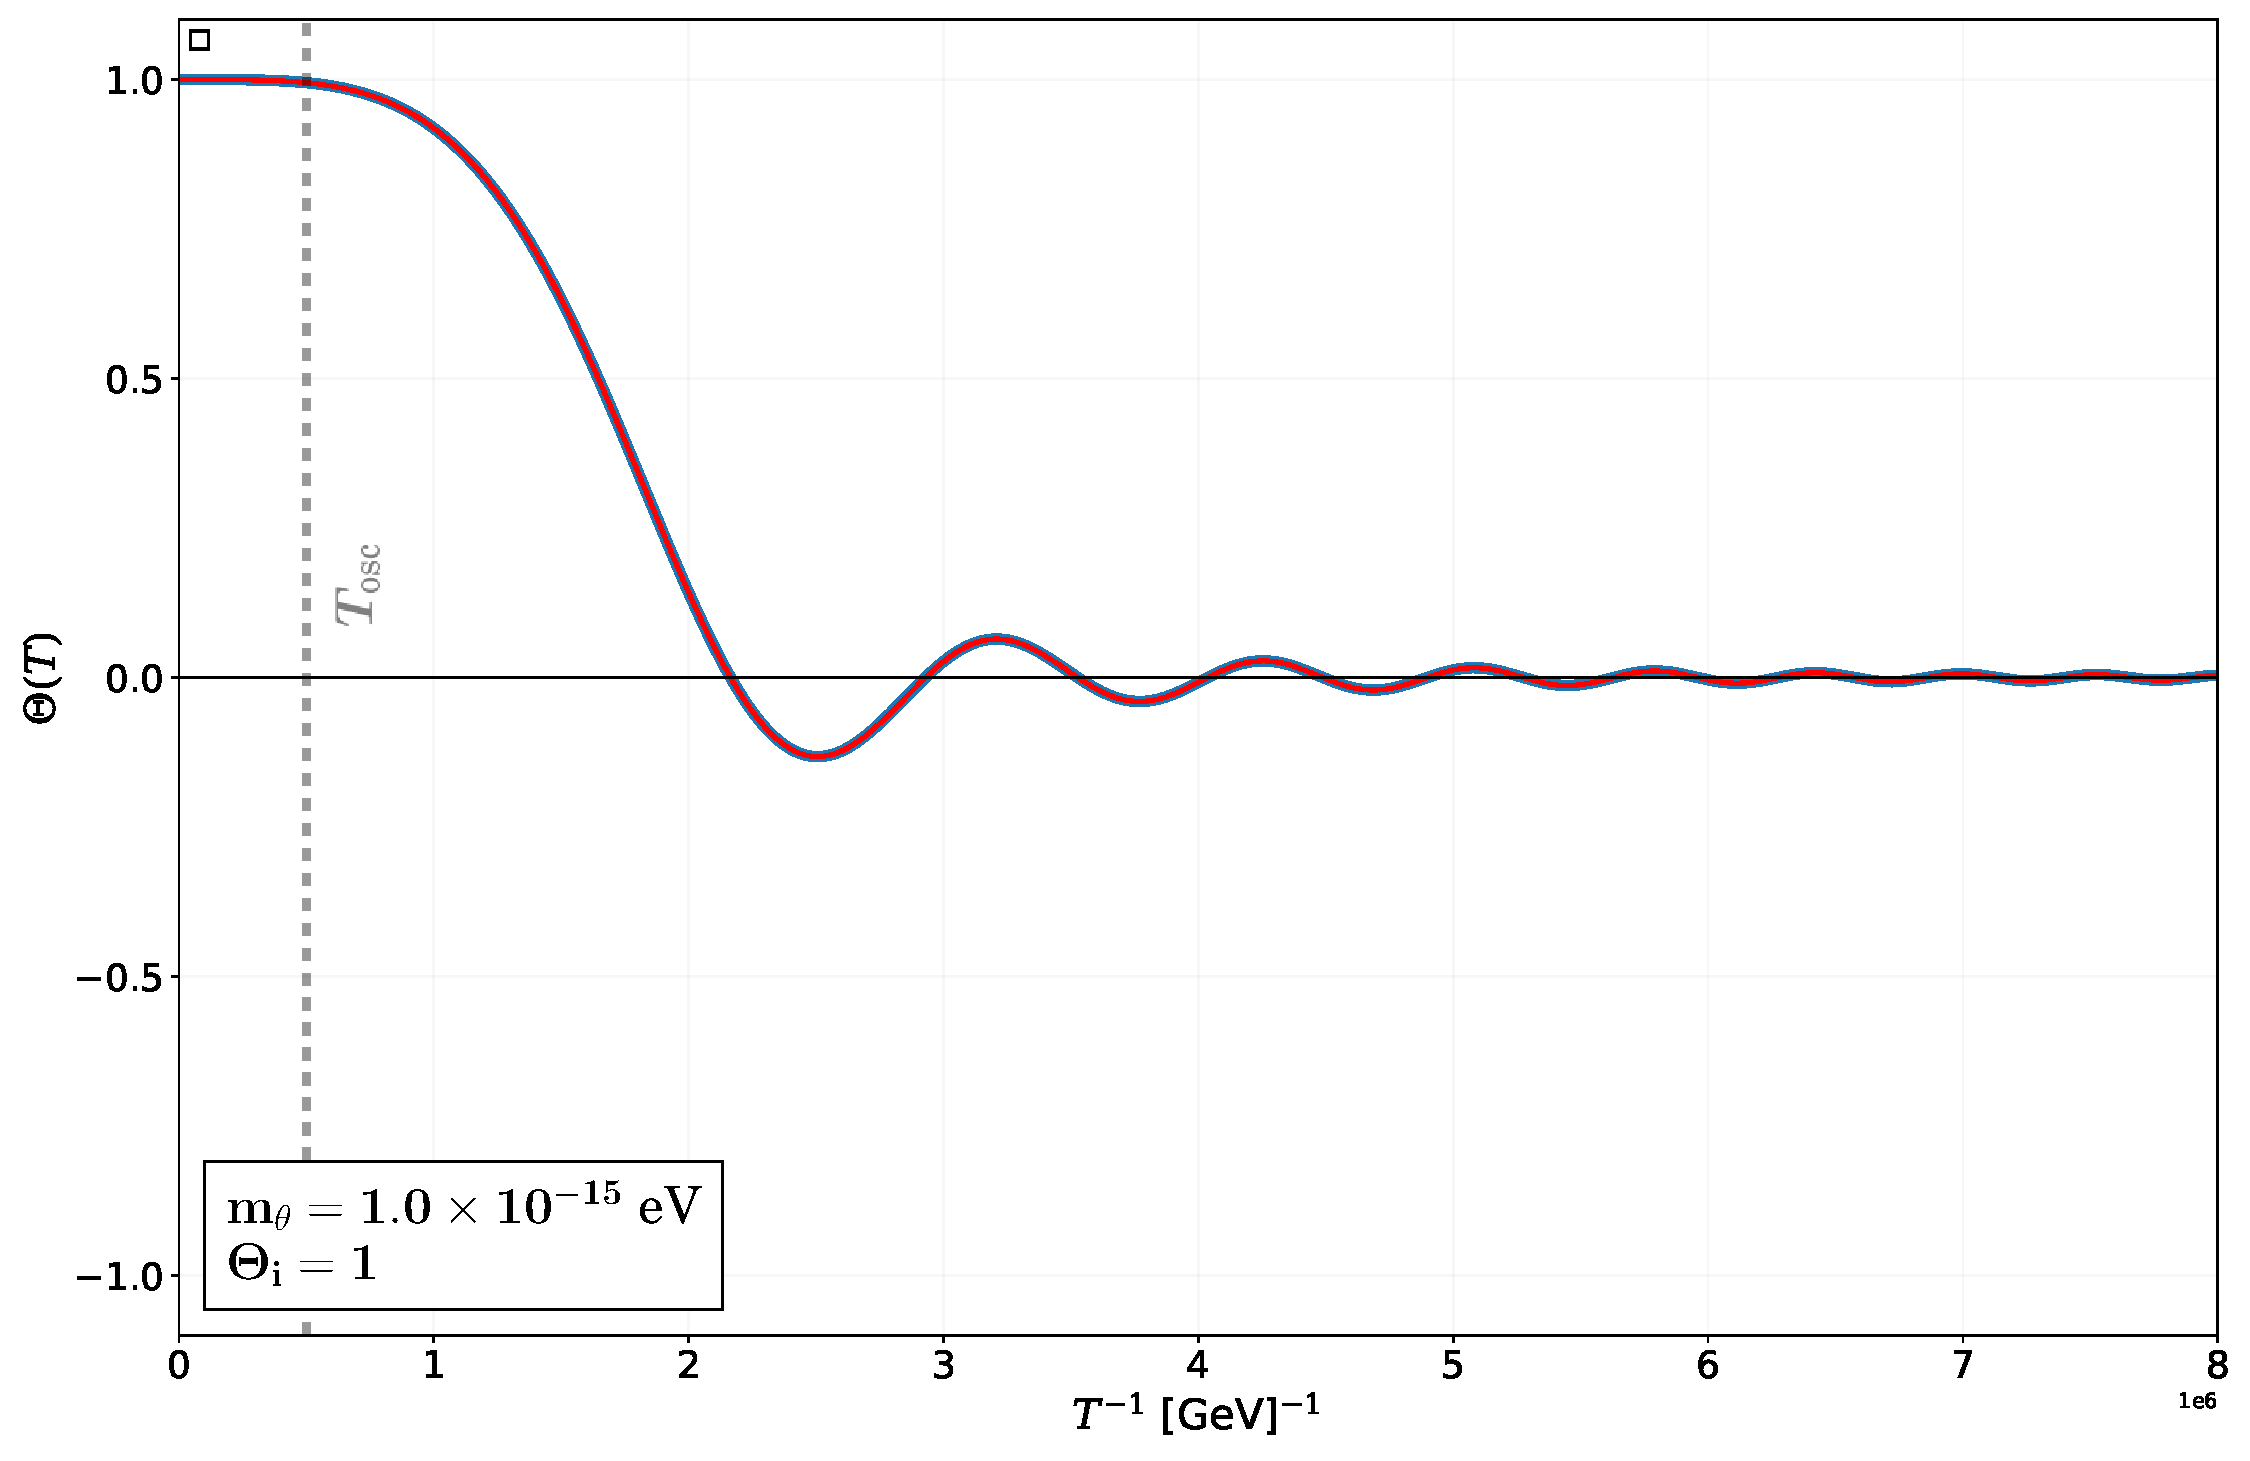
\includegraphics[width=.7\textwidth]{Figures/motion.pdf}
        \caption{Solution of the equation of motion}
        \label{fig:rot}
    \end{figure}
\end{frame}

\begin{frame}{Relic Density of pNGB}
    \[\Scale[0.7]{\Omega^0_\theta h^2=0.11\left(\dfrac{m_\theta}{10^{-14}\si{\eV}}\right)^{1/2}\left(\dfrac{v_\sigma}{\sqrt{50}\times10^{17}\si{G\eV}}\right)^{2}\left(\dfrac{\Theta_\textrm{osc}}{10^{-3}}\right)^{2}\left(\dfrac{3.91}{g_{*s}(T_\textrm{osc})}\right)\left(\dfrac{g_*(T_\textrm{osc})}{3.36}\right)^{3/4}}\]
 %
	\begin{figure}[H]
	\centering
	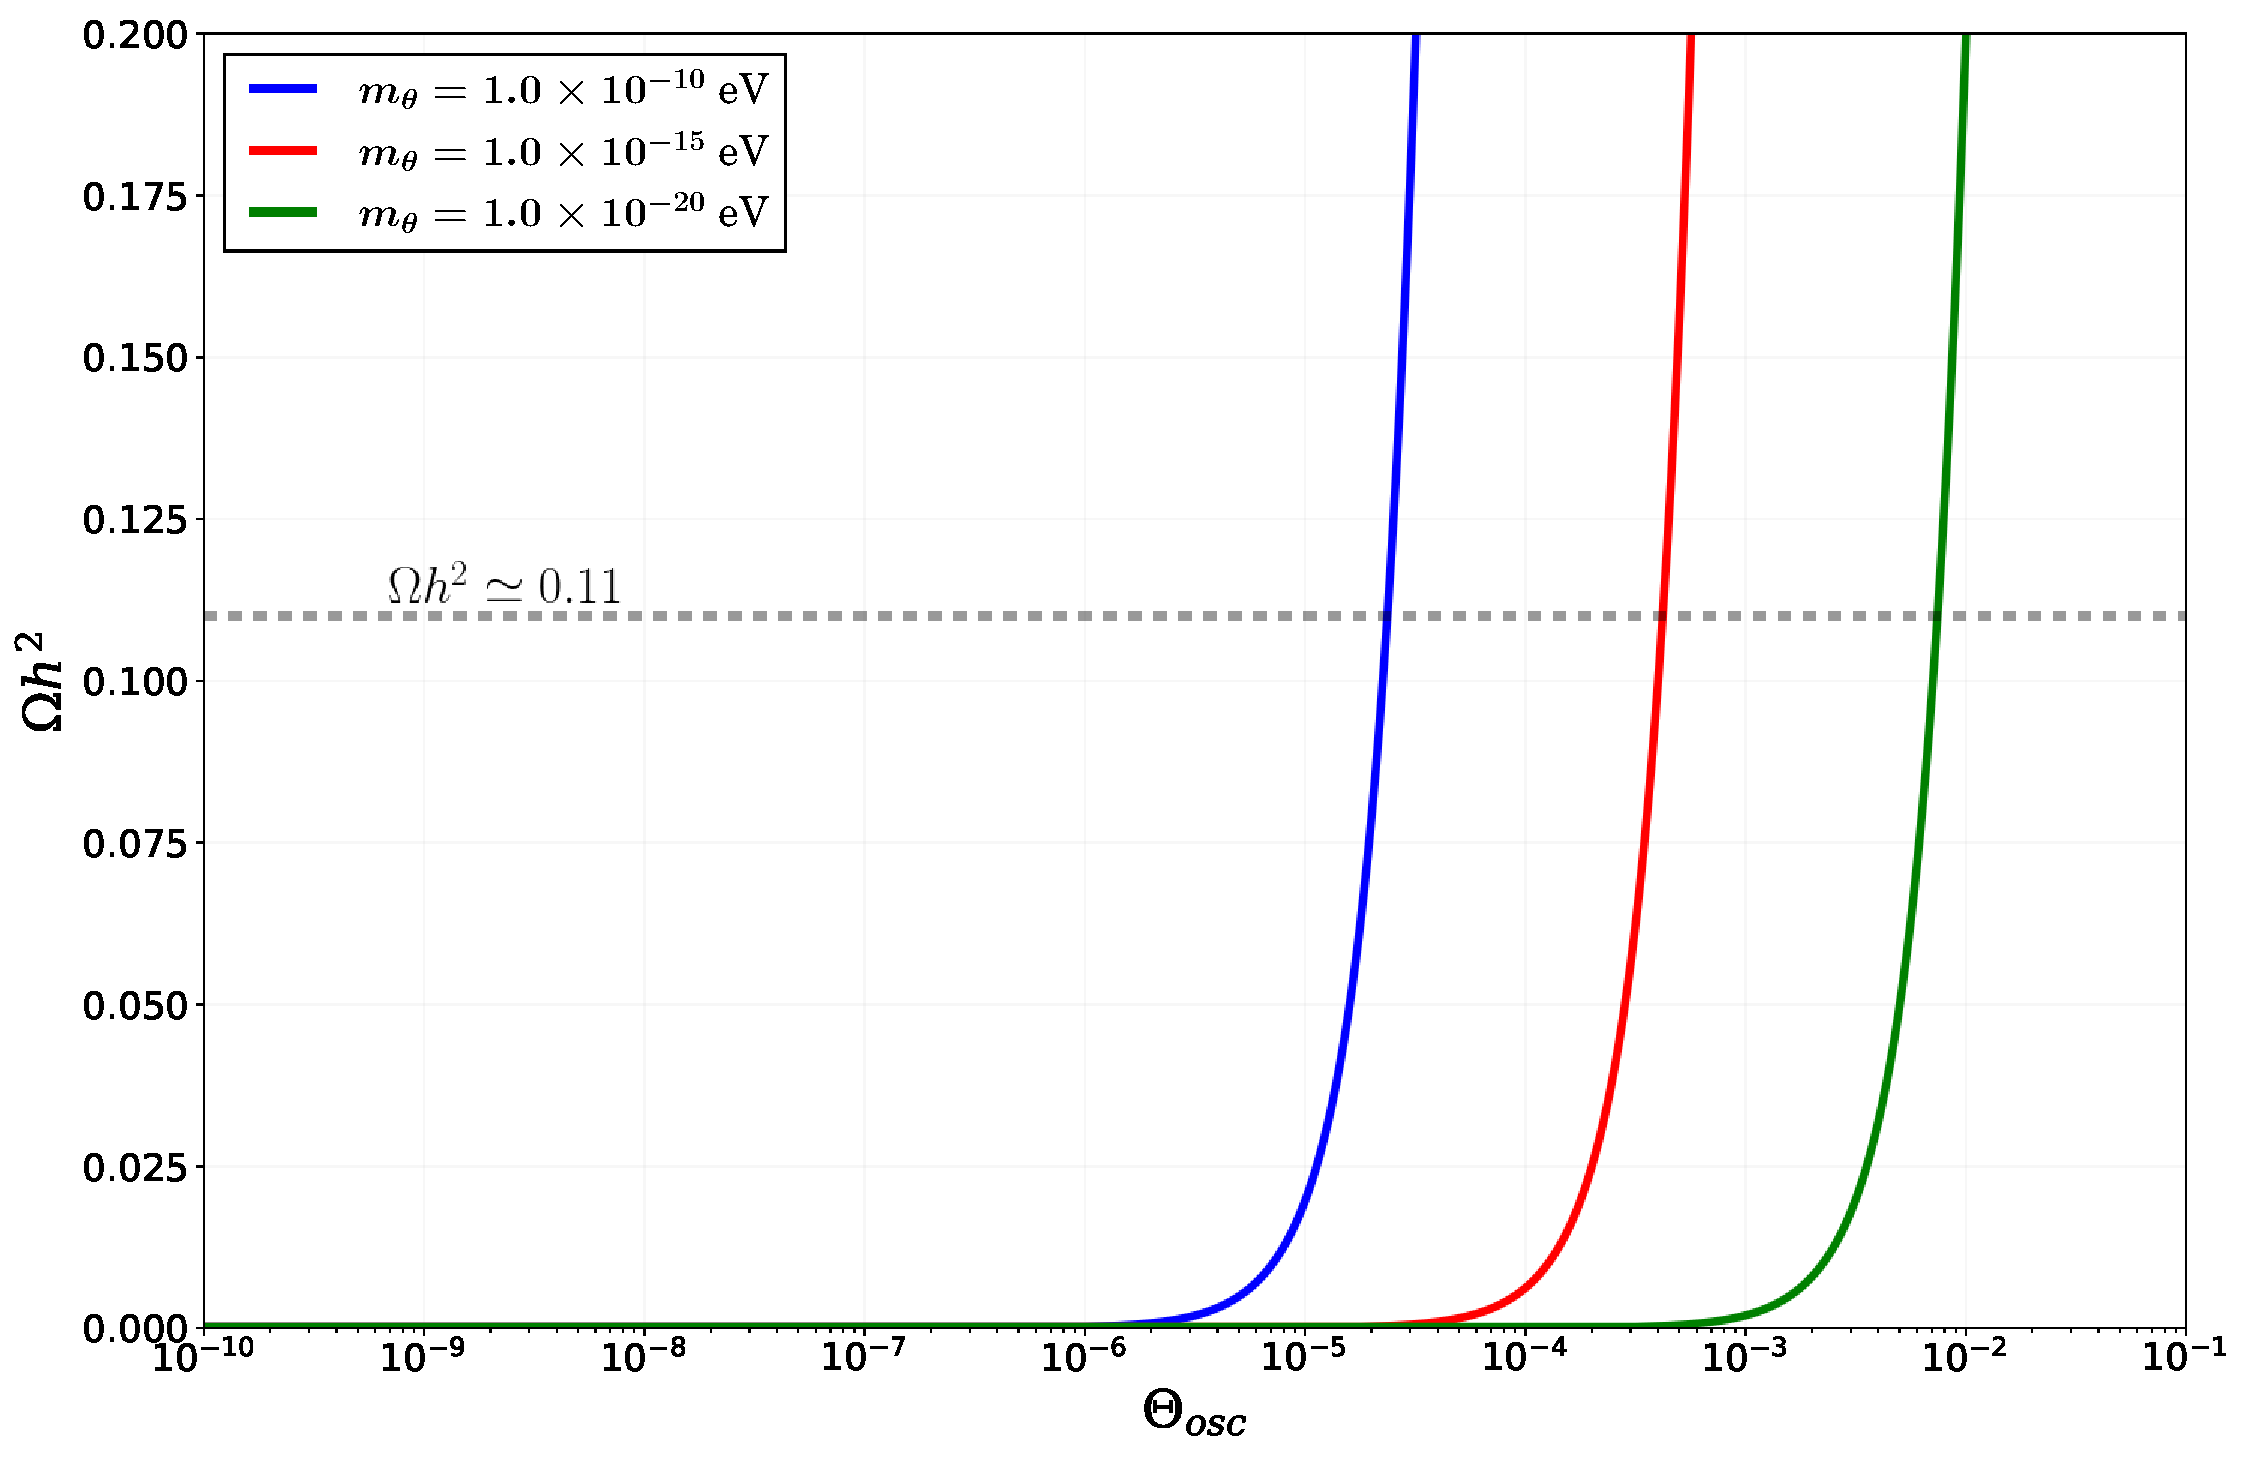
\includegraphics[width=0.6\linewidth]{Figures/relic_density.pdf}
	\caption{Relic density change with the initial Misalignment angle $\Theta_\textrm{osc}$, with $v_\sigma=3\times 10^{18}$, for various values of $m_\theta$\,.}
	\label{fig:relicdesity}
	\end{figure}
\end{frame}
 
